\documentclass[12pt]{article}
%\documentclass[border=0.1cm]{standalone}
\usepackage{wasysym}
\usepackage{phonenumbers}
\usepackage{marvosym }
\usepackage{xcolor}
\usepackage{comment}
\usepackage{pdfpages}
\usepackage[paperwidth=8.5in,paperheight=11in,margin=0.5in]{geometry} 
\usepackage[UKenglish]{babel}
\usepackage[UKenglish]{isodate}% http://ctan.org/pkg/isodate
\usepackage{hyperref}
\usepackage[activate={true,nocompatibility},final,tracking=true,kerning=true,spacing=true,factor=1100,stretch=10,shrink=10]{microtype}
\frenchspacing
\usepackage[nodayofweek,level]{datetime}
\usepackage{calc,url}
\newcounter{qz}\setcounter{qz}{0}
\newcommand{\qz}{%\
\setcounter{qz}{\value{qz}+1}
\textbf{In-class  \theqz} \,}

\newcounter{hw}\setcounter{hw}{0}
\newcommand{\hw}{%\
\setcounter{hw}{\value{hw}+1}
\textbf{HW \thehw}}

\newcounter{ex}\setcounter{ex}{0}
\newcommand{\ex}{%\
\setcounter{ex}{\value{ex}+1}
Exam \theex}

\usepackage[T1]{fontenc} 
\usepackage{fourier}
%\usepackage{tgschola} %to look retro
\newenvironment{mypar}[2]
  {\begin{list}{}%
    {\setlength\leftmargin{#1}
    \setlength\rightmargin{#2}}
    \item[]}
  {\end{list}}


\newcounter{wk}\setcounter{wk}{0}
\newcommand{\wk}{%\
\setcounter{wk}{\value{wk}+1}
\thewk \,\,}

\usepackage[nomessages]{fp}% http://ctan.org/pkg/fp


\usepackage{enumerate}
\usepackage{graphicx}

\usepackage{paralist}
\renewenvironment{description}[0]{\begin{compactdesc}}{\end{compactdesc}}

\newenvironment{alphalist}{
  \begin{enumerate}[(a)]
    \addtolength{\itemsep}{-0.5\itemsep}}
  {\end{enumerate}}
  \cleanlookdateon% Remove ordinal day reference
  \newcommand{\RomanNumeralCaps}[1]
      {\MakeUppercase{\romannumeral #1}}

\usepackage{xspace}
\makeatletter
\DeclareRobustCommand{\maybefakesc}[1]{%
  \ifnum\pdfstrcmp{\f@series}{\bfdefault}=\z@
    {\fontsize{\dimexpr0.8\dimexpr\f@size pt\relax}{0}\selectfont\uppercase{#1}}%
  \else
    \textsc{#1}%
  \fi
}
\newcommand\AM{\,\maybefakesc{am}\xspace}
\newcommand\PM{\,\maybefakesc{pm}\xspace}
\makeatother

 \newcommand{\coursename}{Advanced Calculus I}
\newcommand{\coursenumber}{MATH 460}
\newcommand{\sectionnumber}{01}
\newcommand{\term}{Fall }
\newcommand{\room}{Discovery Hall, room  386}
\newcommand{\meetingtime}{This class meets Monday, Wednesday, and Friday  from 
	9:05\AM -- 9:55\AM}
\newcommand{\officehours}{ Monday, Wednesday, and Friday 10:00\AM -- 11:00\AM,
    Tuesday and Thursday 9:30\AM -- 11:00\AM, and by appointment.}

    \newcommand{\finaldateandtime}{\printdate{14/12/\the\year} 8:00\AM{} -- 10:00 \AM}
\begin{document}
\cleanlookdateon% Remove ordinal day reference
\shortdate
\printyearoff
\large
\begin{center}
    \textbf{\coursename}  \\
    {\coursenumber--\sectionnumber} \\
     {\term \the\year} \\
\end{center}

\vskip0.25in
\normalsize


\begin{center}
\begin{description}
    \item[Instructor:] Barton Willis, PhD, Professor of Mathematics
    \item[Office:]  Discovery Hall, Room 368
    \item[\phone:]   \phonenumber[country=US]{3088658868}
    \item[\Email:]    \href{mailto:willisb@unk.edu}{willisb@unk.edu}
    \item[Zoom:] 616 568 5706
    \item[Office Hours:] \officehours
  \end{description}
\end{center}



\subsubsection*{Important Dates}

\begin{mypar}{0.25in}{0.25in} 

      \textbf{First Homework due} \dotfill  \printdate{27/8/\the\year}  \\
       \textbf{Exam 1} \dotfill \printdate{23/9/\the\year}  \\
    \textbf{Exam 2} \dotfill  \printdate{4/11/\the\year} \\
    \textbf{Exam 3} \dotfill \printdate{2/12/\the\year} \\
      \textbf{Final exam} \dotfill  \finaldateandtime
\end{mypar}



\subsubsection*{Grading}

Your course grade will be based on weekly homework sets, three midterm exams, and a comprehensive 
final exam; specifically:
\begin{mypar}{0.25in}{0.25in}
    \textbf{Weekly Homework:}  \emph{12 fifteen point assignments}  \dotfill 180 (total) \\
    \textbf{Mid-term exams 1,2, and 3:} \emph{100 points each} \dotfill 300 (total)\\
      \textbf{Comprehensive Final exam} \dotfill 150 (total)
\end{mypar}
If we end the term with less than 180 points for homework,  your homework point total will be scaled to a total of 180. 

\FPeval{\points}{round(180+300+150,0)}

\FPeval{\F}{round(\points*0.6-1,0)}
\FPeval{\Dm}{round(\points*0.6,0)}
\FPeval{\D}{round(\points*0.633,0)}
\FPeval{\Dp}{round(\points*0.666,0)}

\FPeval{\Cm}{round(\points*0.7,0)}
\FPeval{\C}{round(\points*0.733,0)}
\FPeval{\Cp}{round(\points*0.766,0)}

\FPeval{\Bm}{round(\points*0.8,0)}
\FPeval{\B}{round(\points*0.833,0)}
\FPeval{\Bp}{round(\points*0.866,0)}

\FPeval{\Am}{round(\points*0.9,0)}
\FPeval{\A}{round(\points*0.933,0)}
\FPeval{\Ap}{round(\points*0.966,0)}

The following table shows the \emph{minimum} number of points (out of \points) that
are required for each of the twelve letter grades D- through A+. For
example, a point total of \Bp\/  points will earn you a grade of B+,  and 
a point total of \Am\/ points will earn you a grade of A-. If you earn a point
total of \F\/  or less, you a failing course grade.
 
 \vspace{0.1in}
     \begin{minipage}{5.5in}
  \centering 
\begin{mypar}{0.25in}{0.25in}
    \begin{minipage}{2.5in}
        D-  \dotfill \Dm \\
        D \dotfill \D \\
        D+ \dotfill \Dp \\
        C- \dotfill \Cm  \\
        C \dotfill \C \\
        C+ \dotfill \Cp 
        \end{minipage}
    \phantom{xxx}
    \begin{minipage}{2.5in}
        B- \dotfill \Bm \\
        B \dotfill  \B \\
        B+ \dotfill  \Bp\\
        A- \dotfill  \Am \\
        A \dotfill  \A \\
        A+ \dotfill  \Ap
    \end{minipage}
\end{mypar} 
\end{minipage}

\subsubsection*{Class meeting time and place}

\meetingtime in \room.

\subsubsection*{Course Resources}

Our textbook is \emph{An Introduction to Analysis}, 2nd edition, Waveland Press, Prospect Heights, Illinois, 2002 (ISBN 13: 978-1-57766-232-7) by James Kirkwood. The book by the same author and title, but published by PWS Publishing Company (Boston, 1995, ISBN 13:
0-534-94422-1) is identical.

 Some homework assignments for this course will need to be typeset. To do this, you will need to create a \emph{no cost} 
account on Overleaf (\url{https://www.overleaf.com/}).   For a  tutorial for using Overleaf, see \url{https://www.overleaf.com/tutorial}.



\subsubsection*{Course Calendar}

Generally, we'll adhere to the scheduled exam dates even if we are ahead or behind with coursework.  
When we are ahead or behind, the topics on the exams will be appropriately adjusted.  


\vspace{0.1in}
\noindent \textbf{Notices:}


\begin{alphalist}
   \item \emph{Exams will be given on  \textbf{Friday} of the week they are assigned.}
   

    \item Homework (labelled \textbf{HW}) will be due one minute before midnight on  Saturday of the week they are assigned.  

    \item The final exam will be given on \finaldateandtime.
    
\end{alphalist}

\vspace{0.1in}

\begin{center}
    \small
\begin{tabular}  {|l|l|l|l|l|}
\hline
{\bf Week}  & \textbf{Week Starting} &  {\bf Section(s)} & {\bf Topic(s)} & \textbf{Assessments} \\
\hline \hline 
\wk    &  \printdate{22/8/\the\year} &     & Logic, Proof methods, and Overleaf & \hw  \\
\wk    & \printdate{29/8/\the\year}   &  \S1.1 -- 1.3  & Sets, Functions, Real numbers, Completeness   & \hw  \\
\wk    & \printdate{5/9/\the\year}&     \S2.1 -- \S2.2  & Sequences \& Subsequences    &  \hw \\
\wk    & \printdate{12/9/\the\year}&     \S2.1 -- \S2.2  & Sequences \& Subsequences    &  \hw \\
\wk    & \printdate{19/9/\the\year}   &  \S2.3  & Bolzano-Weierstrass    &   \textbf{\ex}          \\ \hline
\wk    & \printdate{26/9/\the\year} &  \S3.1    &  Topology    &  \hw \\ 
\wk    & \printdate{3/10/\the\year}    & \S3.1  &   Topology  &    \hw  \\
\wk    & \printdate{10/10/\the\year}     & \S4.1  & Limits and Continuity & \hw \\
\wk    & \printdate{17/10/\the\year}   & \S4.1  & Limits and Continuity     & \hw   \\
\wk   &  \printdate{24/10/\the\year}   & \S4.2 & Monotone and Inverse Functions     & \hw \\ 
\wk   &  \printdate{31/10/\the\year}      &   \S5.1 & Derivatives   &  \textbf{\ex} \\ \hline
\wk   &  \printdate{7/11/\the\year}   &   \S5.1 &  Derivatives   & \hw  \\
\wk   & \printdate{14/11/\the\year}  & \S5.2    & Some Mean Value Theorems   &  \hw   \\
\wk   & \printdate{21/11/\the\year} & \S6.1  & The Riemann Integral    & \hw \\
\wk   & \printdate{28/11/\the\year}    &  \S6.2  & The Riemann Integral     &   \textbf{\ex}    \\
\wk   & \printdate{5/12/\the\year}   &       &  Catch up or Review     &    \\ \hline
 \wk   & \printdate{12/12/\the\year}     &     &    \hfill  & \textbf{ Final Exam}  \\  \hline
   
\end{tabular}
\end{center}


\subsubsection*{University Policies}

Please see \url{https://www.unk.edu/academic_affairs/asa_forms/course-policies-and-resources.php}.

\subsubsection* {Policies}

Unless an assessment is \emph{explicitly} stated to be a group project,  \emph{all work you turn in for a grade must be your own.}  If you need assistance in completing a homework assignment, you may ask me for help. Googling for answers, seeking help from the Learning Commons or other faculty members,  or using solution keys from previous terms (either from UNK or other universities) is also prohibited.  Violation of these rules will result in earning a grade of zero on the assessment. Each homework assignment you turn in for a grade must include the statement:

\begin{quote}
\fbox{I have neither given nor received unauthorized assistance on this assignment.}
\end{quote}
 If two assignments are so similar that only collaboration could explain their similarities, both assignments will receive a grade of zero.  Using unauthorized materials or communication devices (cell phone, for
example) while taking a test will earn you a grade of zero on that assessment.  

 

\begin{enumerate}

\item Regular in person class attendance is required. If you are ill or need to miss class due to athletics, please let me know ahead of time, and I will make an effort to put the class on Zoom.

\item For examinations and in class assignments, show your work.  \emph{No credit will be given for multi-step problems without the necessary work. Your solution must contain enough detail
so that I am convinced that you could correctly work any similar problem.} Also erase or clearly mark any work you want me to ignore; otherwise,
I'll grade it.  

\item The work you turn in is expected to be \emph{accurate, 
complete, concise, neat}, and \emph{well-organized}.  
\emph{You will not earn full credit on work that falls short of 
these expectations.}

\item Class cancellations due to weather or illness or other 
unplanned circumstances may require that we make  adjustments
to the course calendar, exam dates, and due dates or specifics for 
course assessments. 


\item Extra credit is not allowed. 



\item For examinations, you may use a teacher provided quick reference sheet, 
but no other reference materials. You may also use a pencil, eraser, 
and a scientific calculator. For examinations, your phone and all such
devices must be turned off and \emph{out of sight}. 

\item Generally, if you are ill or absent for any reason (including 
athletics), you must turn in your in class work on time. Permission to
turn in work late must be made in advance, otherwise late in class work 
will count zero points.


 

\item During class time, please refrain from using electronic devices. If your 
device usage distracts your classmates, I will ask you to put it away. If it's my 
impression that you are often not paying attention in class, I reserve the right to 
decline to help you during office hours.

\item The final examination will be \emph{comprehensive} and it will be given 
during the  time scheduled by the University. Except for \emph{extraordinary circumstances}
you must take the exam at this time.
 
\item If you have questions about how your work has been graded, make an appointment with me immediately.


\item Please regularly check Canvas  to verify that your scores have 
been recorded correctly.  If I made a mistake in recording one of
your grades, I'll correct it provided you saved your paper.



\end{enumerate}
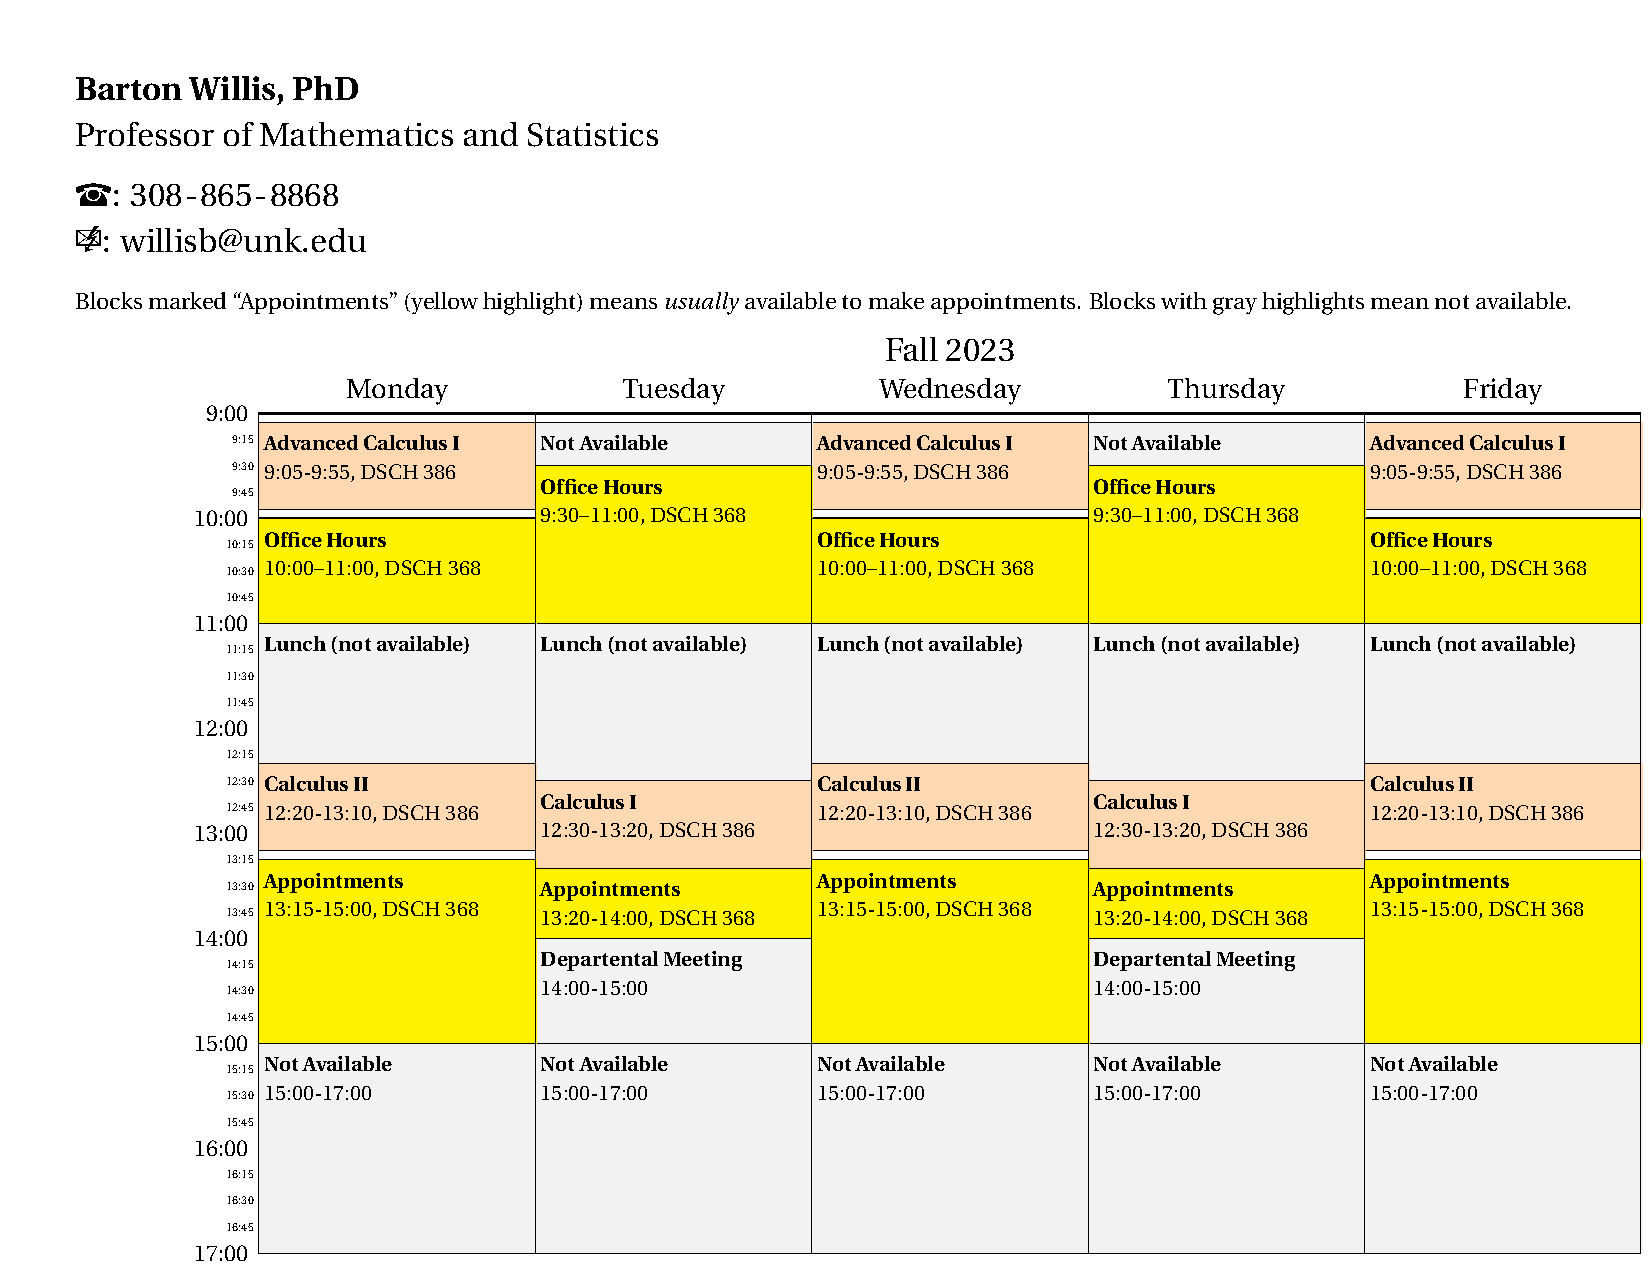
\includepdf[pages={1-},angle=90]{door_schedule.pdf}  
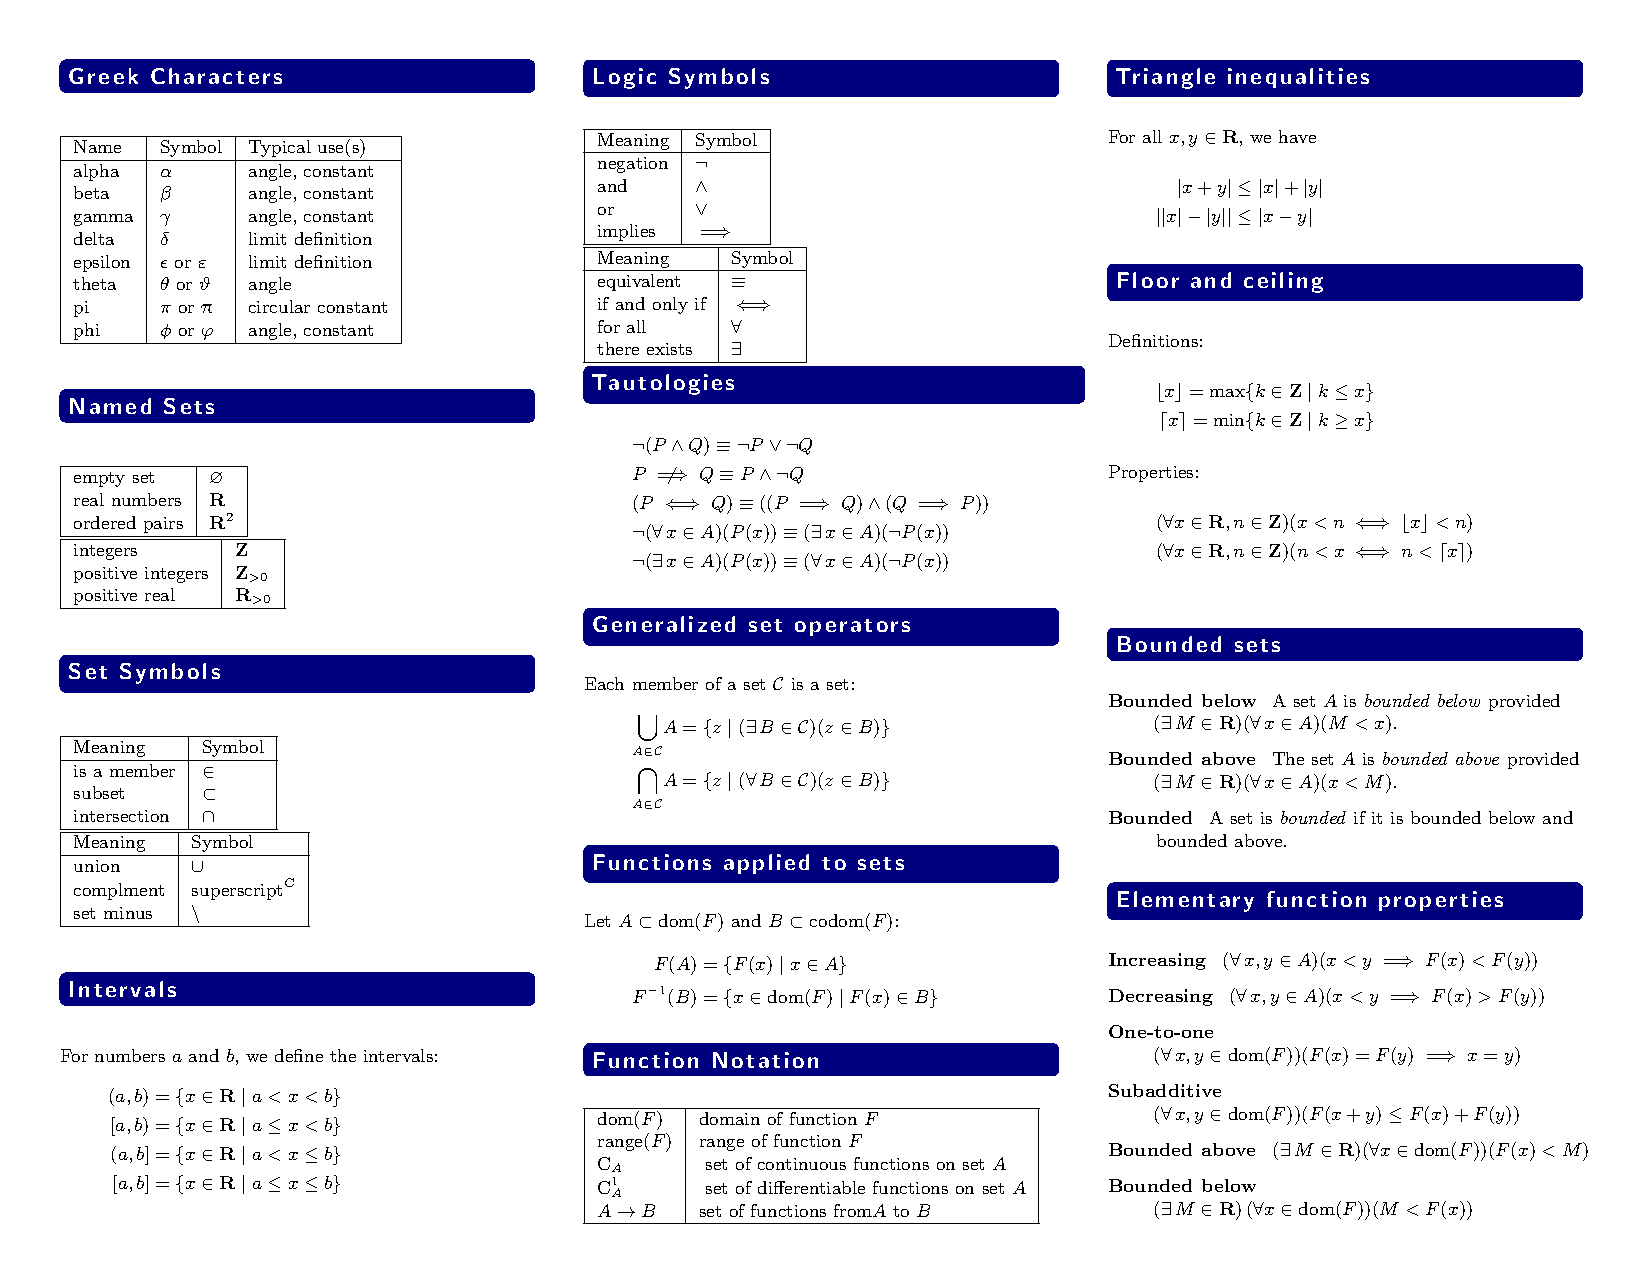
\includepdf[pages={1-},angle=90]{analysis-quick-reference.pdf} 
\end{document}

